\section{Setup}
%%%%%%%%%%%%%%%%%%%%%%%%%%%%%%%%%%%%%% FRAME 0 %%%%%%%%%%%%%%%%%%%%%%%%%%%%%%%%%%%%%%%%%%%%%%%%
{
	\setbeamertemplate{footline}{}
	\begin{frame}
		\begin{tikzpicture}[remember picture,overlay]
			\node[at=(current page.center)] {
				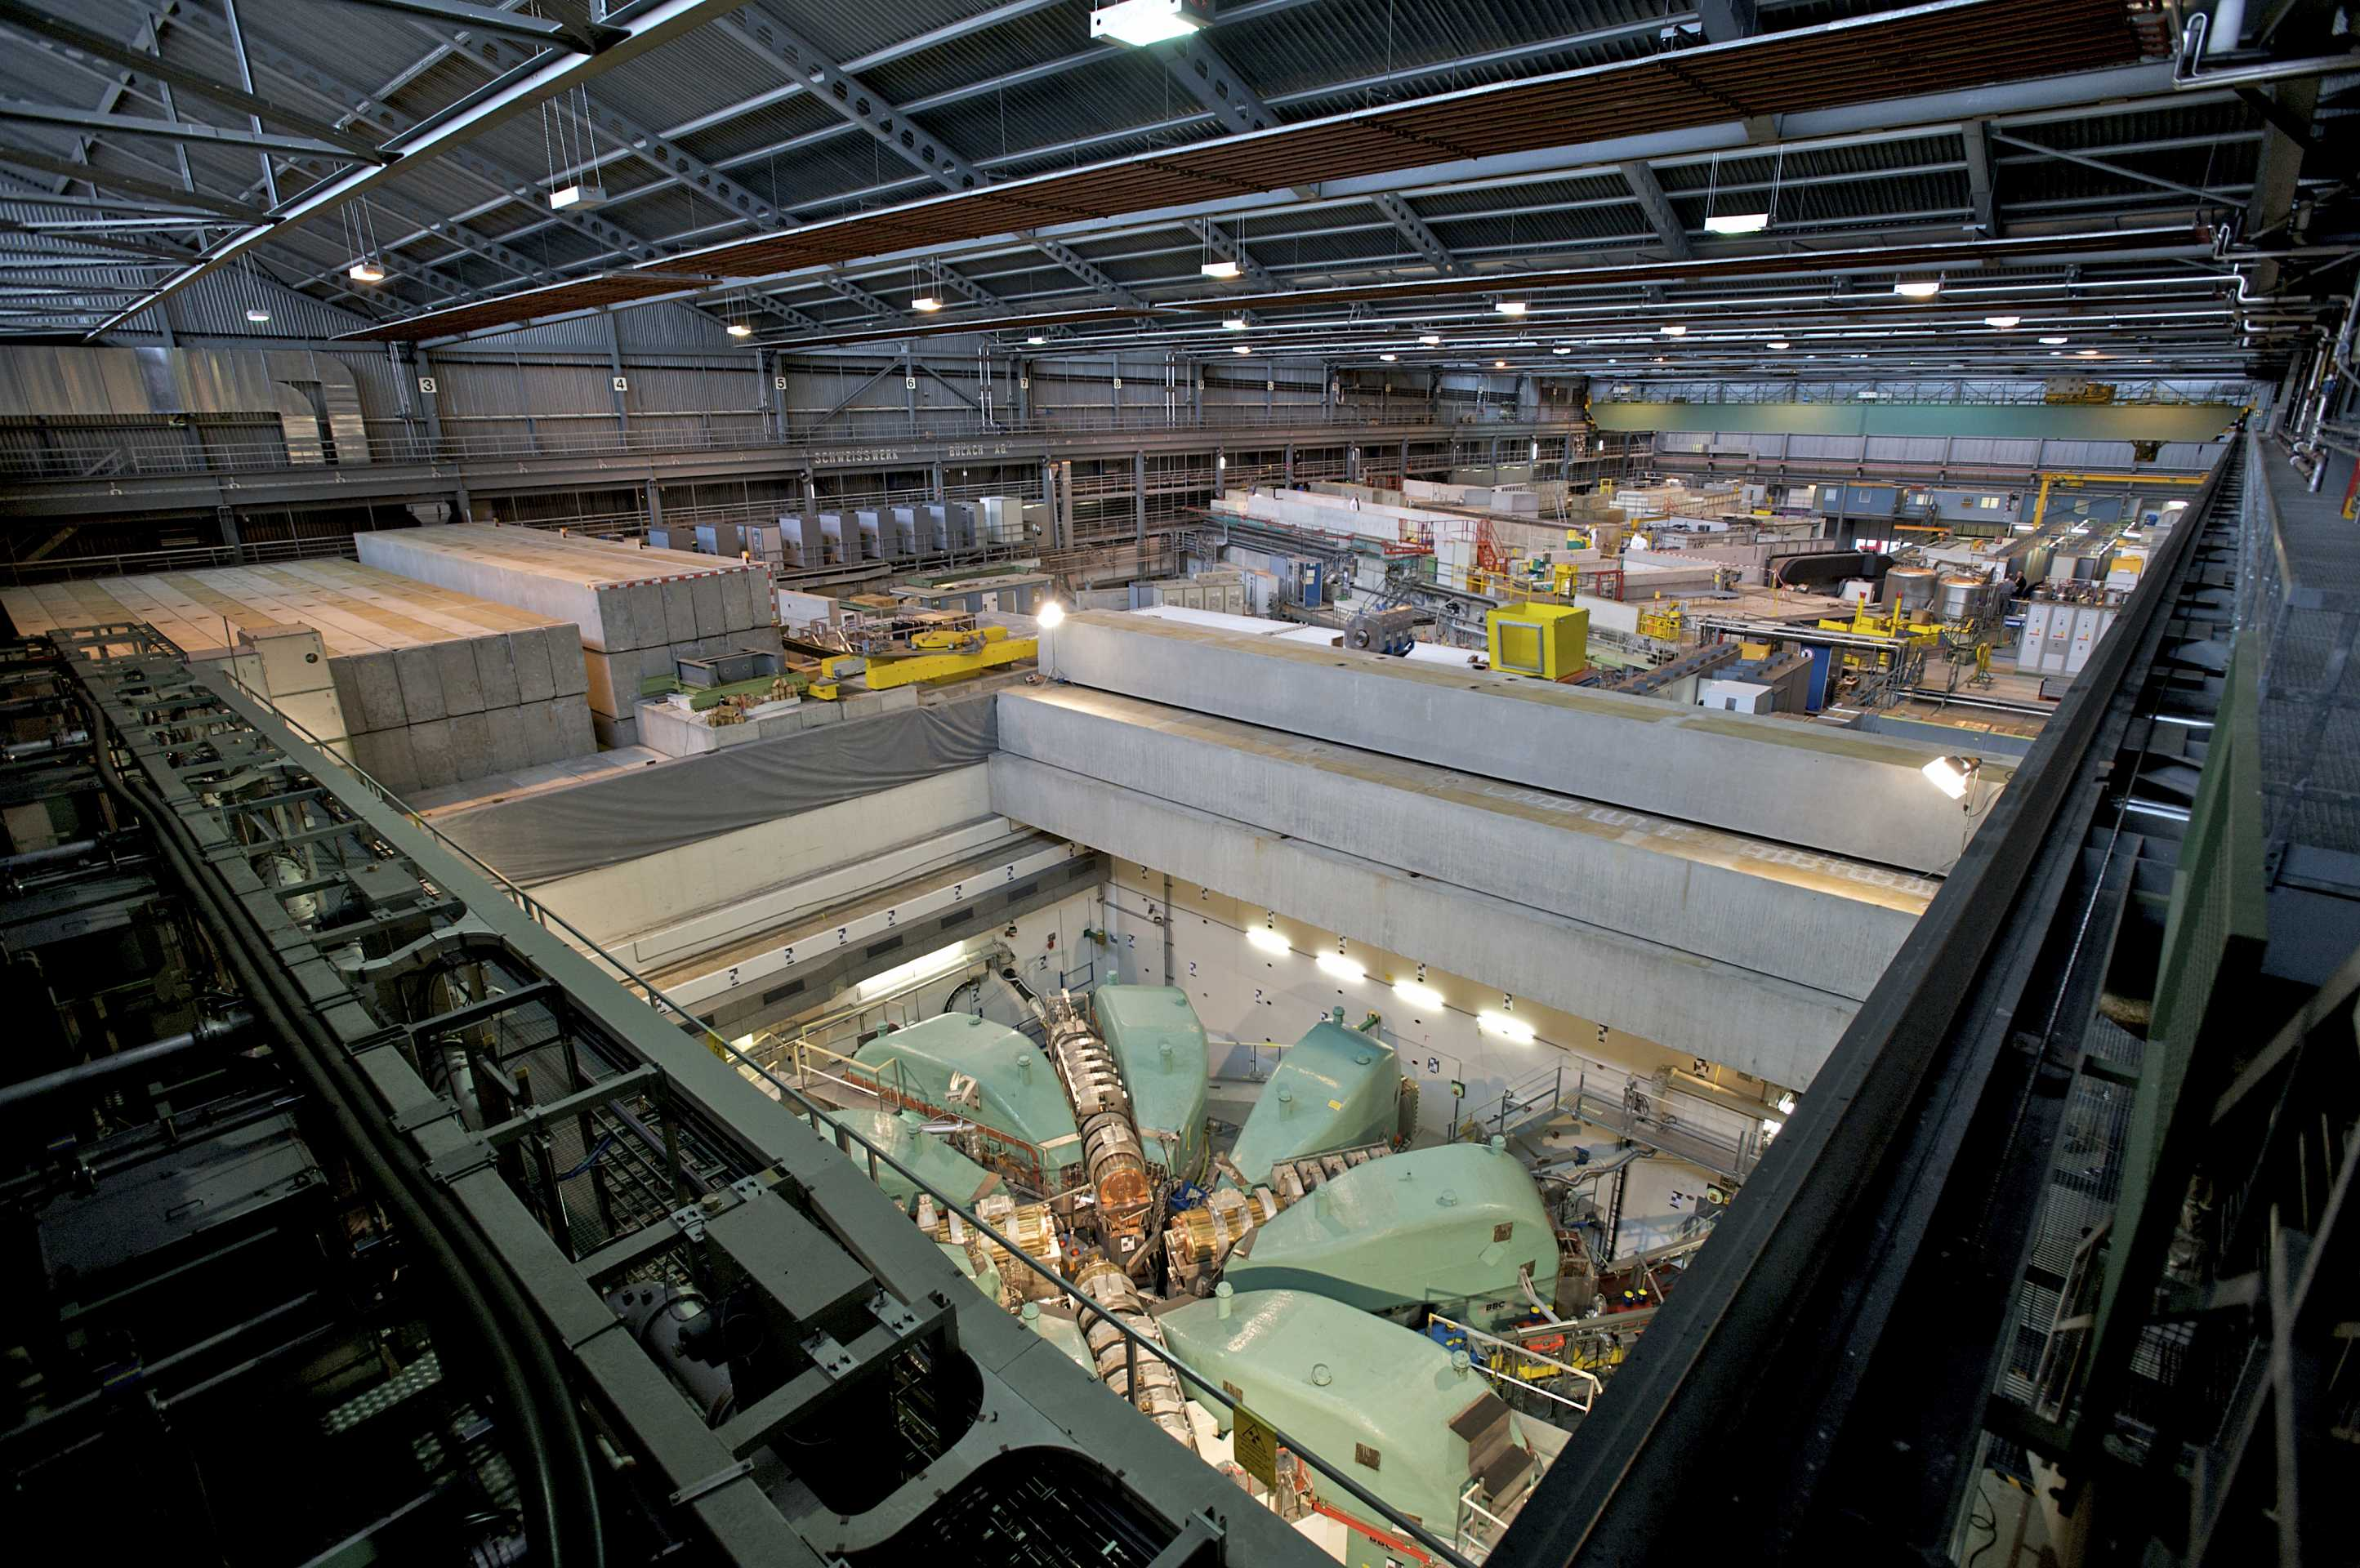
\includegraphics[width=1.15\paperwidth]{Cyclo2}};
		\end{tikzpicture}
		
	\end{frame}
}
%%%%%%%%%%%%%%%%%%%%%%%%%%%%%%%%%%%%%% FRAME 1 %%%%%%%%%%%%%%%%%%%%%%%%%%%%%%%%%%%%%%%%%%%%%%%%
\subsection{PSI Experimental Hall}
\begin{frame}{Test Site}

	\vspace*{-10pt}
	\begin{itemize}\itemfill
		\item High Intensity Proton Accelerator (HIPA) at PSI (Cyclotron) \ra beam line PiM1 
		\item clean positive pion beam (\SI{\sim98}{\%} $\uppi^+$) with momentum of \SI{260}{\mega\electronvolt\per c} 
% 		\begin{itemize}
% 			\item \sfrac{3}{4} smaller signals than at CERN! (\SI{120}{\giga\electronvolt\per c})
% 		\end{itemize}
		\item \good{tunable particle fluxes from \orderof{\SI{1}{\kilo\hertz\per cm^2}} to \orderof{\SI{10}{\mega\hertz\per cm^2}}} with collimators
		\item \bad{significant multiple scattering \ra worsens resolution}
	\end{itemize}
	
	\subfigs[\subfig[.36]{.48}{Cyclo1}]{\subfig[.3]{.5}{Cyclo3}}{\subfig[.22]{.25}{Target}}\vspace*{-10pt}

\end{frame}

%%%%%%%%%%%%%%%%%%%%%%%%%%%%%%%%%%%%%% FRAME 2 %%%%%%%%%%%%%%%%%%%%%%%%%%%%%%%%%%%%%%%%%%%%%%%%
\subsection{Final}
\begin{frame}{Final Setup}

	\fig{.55}{TelPad}[Modular Beam Telescope]\vspace{-10pt}

	\begin{itemize}\itemfill
		\item 4 tracking planes \ra trigger (fast-OR) with adjustable area (max \SI{8x7.8}{\milli\meter})
		\item diamond pad detectors in between tracking planes
		\item fast scintillator \ra precise trigger timing of \orderof{\SI{1}{\nano\second}}
	\end{itemize}

\end{frame}
%%%%%%%%%%%%%%%%%%%%%%%%%%%%%%%%%%%%%% FRAME 3 %%%%%%%%%%%%%%%%%%%%%%%%%%%%%%%%%%%%%%%%%%%%%%%%
\subsection{Development}
\begin{frame}{Setup Development}

	\fig{.55}{TelSchematics2}[Current Setup (Aug16 - Oct18)]\vspace{-10pt}
	
	\begin{itemize}\itemfill
		\item scintillator \ra precise trigger timing of \orderof{\SI{1}{\nano\second}}
		\item Trigger Unit (TU) \ra strongly simplifying setup
		\item global trigger \ra (Plane 1 AND Plane 2) AND Scintillator
	\end{itemize}
	
\end{frame}
